\documentclass[12pt, a4paper]{report}
\usepackage[utf8]{inputenc}
\newcommand\preamble{
    \usepackage[italian]{babel}
    \usepackage{geometry}
    \usepackage{amsmath}
    \usepackage{amssymb}
    \usepackage{graphicx}
    \usepackage{ulem}
    \geometry{margin=2cm}
    \usepackage{listings}
    \usepackage{titling}
    \usepackage{pgfplots}
    \usepackage{tikz}
    \usetikzlibrary{calc}
    \pgfplotsset{compat=1.18}
    \let\olditemize\itemize
    \renewcommand\itemize{\olditemize\setlength\itemsep{0em}}
}

\newcommand{\tikzmark}[1]{\tikz[baseline,remember picture] \coordinate (#1) {};}
\input{titlePage.tex}  
\preamble

\begin{document}
\customTitlePage{Fondamenti dell'Elaborazione di Segnali e Immagini}{Lorenzo Vaccarecci}{Anno Accademico 2024/2025}{Università degli Studi di Genova}
\newpage
\tableofcontents
\chapter{Introduzione}
\section{Segnali 1D e 2D}
\subsection{Segnali 1D}
Un segnale 1D descrive una grandezza fisica che varia nel tempo, e può essere visto come una funzione di una variabile indipendente: 
\begin{equation*}
    g = f(t)
\end{equation*}
dove $g$ è il valore della grandezza fisica (variabile \textbf{dipendente}), $f$ è la funzione (continua o discreta) e $t$ è la variabile indipendente.\\
Esempi di segnali 1D sono:
\begin{itemize}
    \item Segnali audio: come ad esempio la musica o il parlato.
    \item Segnali ECG
    \item Segnali EEG
    \item Sensori inerziali
    \item \dots
\end{itemize}
\subsection{Segnali 2D}
Un segnale 2D descrive una grandezza fisica che varia nello spazio, e può essere visto come una funzione di due variabili indipendenti.\\
Esempi di segnali 2D sono:
\begin{itemize}
    \item Immagini: utilizzeremo questo termine per indicare una foto a colori o a scala di grigi (ci concentreremo su queste).
    \item Immagini biomediche: come ad esempio le radiografie, le ecografie oppure quelle di una risonanza.
    \item Immagini termiche
    \item Immagini satellitari
    \item Immagini microscopiche
    \item \dots
\end{itemize}
Ciò che hanno in comunque tutte queste immagini è che hanno una matrice di pixel che rappresenta qualcosa, nel nostro caso ogni pixel rappresenta l'intensità luminosa nella posizione $(r,c)$ della matrice.
\section{Segnali a tempo continuo o discreto}
\begin{equation*}
    g = f(t)
\end{equation*}
\subsection{Segnali a tempo continuo}
Nei segnali a tempo continuo $t$ assume valori reali
\begin{figure}[h!]
    \centering
    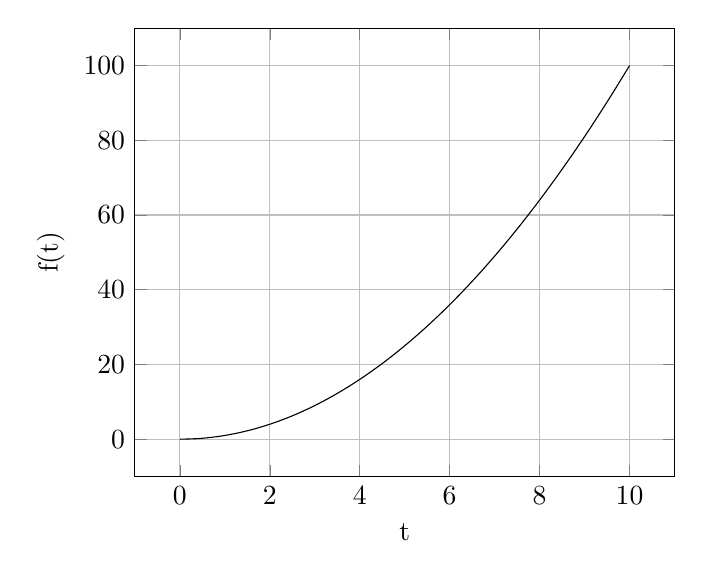
\begin{tikzpicture}
        \begin{axis}[
            xlabel={t},
            ylabel={f(t)},
            grid=major,
        ]
        \addplot[smooth, domain=0:10] {x^2};
        \end{axis}
    \end{tikzpicture}
    \caption{Posso conoscere il valore del segnale in ogni istante di tempo}
\end{figure}
\subsection{Segnali a tempo discreto}
Nei segnali a tempo discreto $t$ assume valori in un sottoinsieme discreto dei numeri reali, come risultato di un'operazione chiamata \textbf{campionamento}.
\begin{figure}[h!]
    \centering
    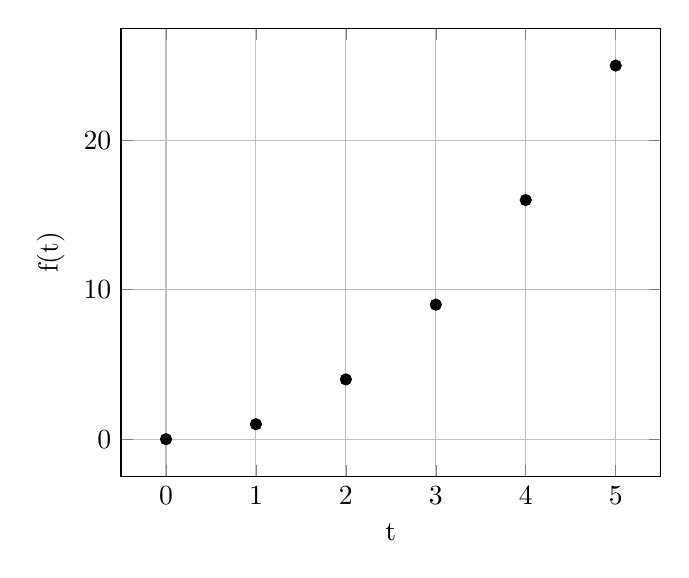
\begin{tikzpicture}
        \begin{axis}[
            xlabel={t},
            ylabel={f(t)},
            grid=major,
            only marks,
        ]
        \addplot[mark=*] coordinates {
            (0,0) (1,1) (2,4) (3,9) (4,16) (5,25)
        };
        \end{axis}
    \end{tikzpicture}
    \caption{Posso conoscere il valore del segnale in certi istanti di tempo}
\end{figure}
\section{Segnali a valori continui o discreti}
\subsection{Segnali a valori continui}
Nei segnali a valori continui $g$ assume valori reali.
\subsection{Segnali a valori discreti}
Nei segnali a valori discreti $g$ assume valori in un sottoinsieme discreto dei numeri reali, come risultato di un'operazione chiamata \textbf{quantizzazione}.
\begin{figure}[h!]
    \centering
    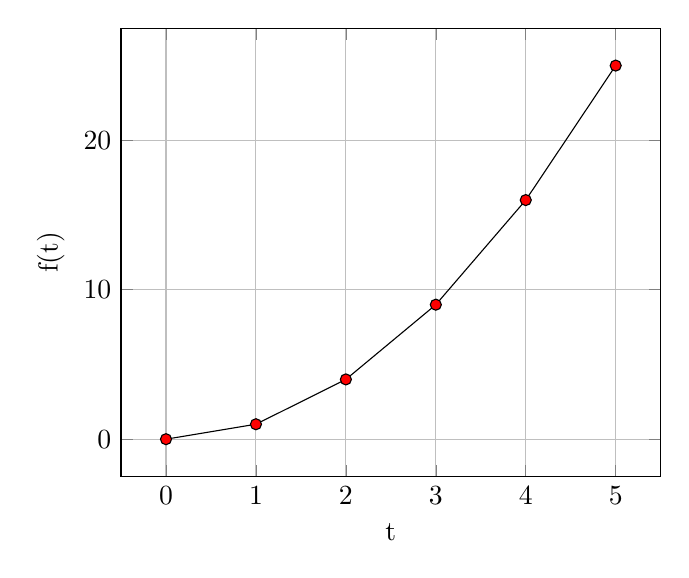
\begin{tikzpicture}
        \begin{axis}[
            xlabel={t},
            ylabel={f(t)},
            grid=major,
        ]
        \addplot[mark=*,mark options={fill=red}, domain=0:5, samples=6] {x^2};
        \end{axis}
    \end{tikzpicture}
    \caption{In rosso i valori \textbf{discreti} di g}
\end{figure}
\section{Analogico e digitale}
\begin{itemize}
    \item \textbf{Segnali analogici}: sono continui sia nel tempo che nei valori.
    \item \textbf{Segnali digitali}: sono discreti sia nel tempo che nei valori.
\end{itemize}
\begin{figure}[h!]
    \centering
    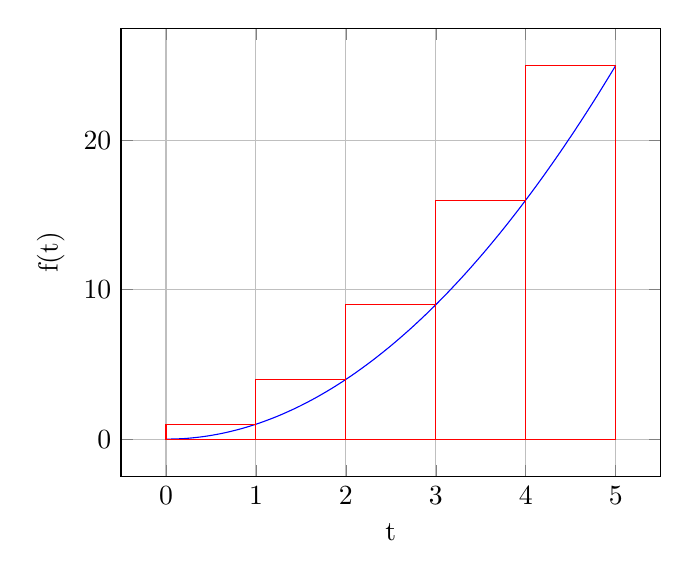
\begin{tikzpicture}
        \begin{axis}[
            xlabel={t},
            ylabel={f(t)},
            grid=major,
        ]
        \addplot[smooth, domain=0:5, color=blue] {x^2};
        \draw[draw=red] (axis cs:0,0) rectangle (axis cs:1,1);
        \draw[draw=red] (axis cs:1,0) rectangle (axis cs:2,4);
        \draw[draw=red] (axis cs:2,0) rectangle (axis cs:3,9);
        \draw[draw=red] (axis cs:3,0) rectangle (axis cs:4,16);
        \draw[draw=red] (axis cs:4,0) rectangle (axis cs:5,25);
        \end{axis}
    \end{tikzpicture}
    \caption{Segnale analogico in blu e segnale digitale in rosso}
\end{figure}
\section{Campionamento}
\begin{equation*}
    v_{s} = \frac{1}{\tau}
\end{equation*}
Dove $v_{s}$ è la frequenza di campionamento e $\tau$ è l'ampiezza dell'intervallo di campionamento. Ovviamente se $\tau$ si avvicina a 0 allora il grafico risultante $f(n\tau)$ sarà più preciso (e vicino a quello continuo) ma userà più risorse per memorizzare i dati.
\subsection{Frequenza ideale di campionamento}
Bisogna stare attenti a non campionare a frequenze troppo basse, altrimenti si incorre nel fenomeno chiamato \textbf{punto di rottura} ossia il grafico risultante apparirà diverso da quello originale.
\begin{figure}[h!]
    \centering
    \includegraphics[width=0.5\textwidth]{Immagini/campionamento.png}
\end{figure}
\\Come possiamo vedere dalla figura l'ultimo grafico risulta essere diverso da quello azzurro (originale), questo perché la frequenza di campionamento non è sufficientemente alta in questo caso si è verificato un punto di rottura.
\newpage
\section{Quantizzazione}
\begin{figure}[h!]
    \centering
    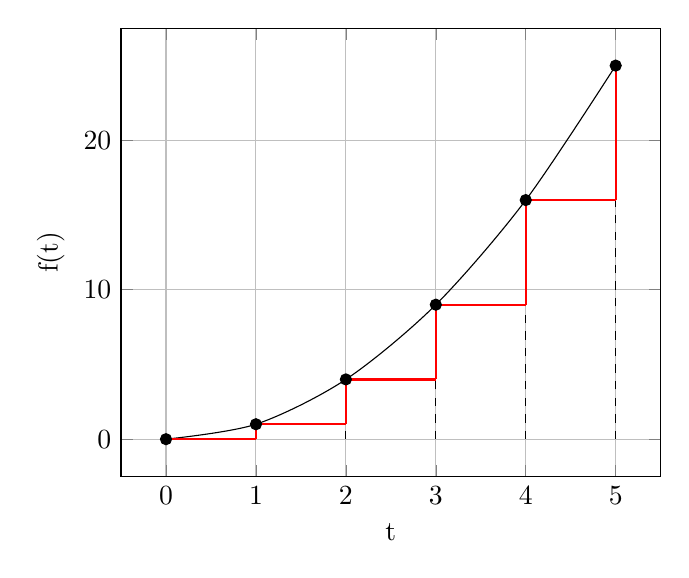
\begin{tikzpicture}
        \begin{axis}[
            xlabel={t},
            ylabel={f(t)},
            grid=major,
        ]
        \addplot[smooth, domain=0:5, mark=*, samples=6] {x^2};
        \draw[dashed] (axis cs:1,0) -- (axis cs:1,1);
        \draw[dashed] (axis cs:2,0) -- (axis cs:2,4);
        \draw[dashed] (axis cs:3,0) -- (axis cs:3,9);
        \draw[dashed] (axis cs:4,0) -- (axis cs:4,16);
        \draw[dashed] (axis cs:5,0) -- (axis cs:5,25);
        \draw[draw=red, thick] (axis cs:0,0) -- (axis cs:1,0);
        \draw[draw=red, thick] (axis cs:1,0) -- (axis cs:1,1);
        \draw[draw=red, thick] (axis cs:1,1) -- (axis cs:2,1);
        \draw[draw=red, thick] (axis cs:2,1) -- (axis cs:2,4);
        \draw[draw=red, thick] (axis cs:2,4) -- (axis cs:3,4);
        \draw[draw=red, thick] (axis cs:3,4) -- (axis cs:3,9);
        \draw[draw=red, thick] (axis cs:3,9) -- (axis cs:4,9);
        \draw[draw=red, thick] (axis cs:4,9) -- (axis cs:4,16);
        \draw[draw=red, thick] (axis cs:4,16) -- (axis cs:5,16);
        \draw[draw=red, thick] (axis cs:5,16) -- (axis cs:5,25);
        \end{axis}
    \end{tikzpicture}
\end{figure}
Partendo da una funzione $f(n\tau)$ quantizziamo i valori associando ad ogni valore $x$ il valore numerico $xk$ che è più vicino ad $x$.
\section{Riepilogo digitalizzazione}
\begin{figure}[h!]
    \centering
    \includegraphics[width=\textwidth]{Immagini/digitalizzazione.png}
\end{figure}
\section{Ripasso: trasformazioni di segnali (1D)}
\subsection{Traslazione}
\begin{equation*}
    f(t-t_{0})
\end{equation*}
\subsection{Scalatura}
\begin{equation*}
    f(\alpha t)
\end{equation*}
\begin{itemize}
    \item $\alpha > 1$ : compressione
    \item $0 < \alpha < 1$ : rilassamento
\end{itemize}
\subsection{Segnali "notevoli"}
\begin{itemize}
    \item \textbf{Segnale rettangolare}: \begin{equation*}
        f(t) = \begin{cases} 
        1 & \lvert t \rvert < \frac{1}{2} \\
        0 & \lvert t \rvert > \frac{1}{2}
    \end{cases}
    \end{equation*}
    \item \textbf{Segnale gradino}: \begin{equation*}
        f(t) = \begin{cases} 
        1 & t > 0 \\
        0 & t < 0
    \end{cases}
    \end{equation*}
    \item \textbf{Segnale impulsivo (o delta di Dirac)}: \begin{equation*}
        \delta(t) = \begin{cases} 
        \infty & t = 0 \\
        0 & t \neq 0
    \end{cases}
    \end{equation*}
\end{itemize}
\subsection{Treno di impulsi equispaziati}
\begin{equation*}
    \delta_{r}(t) = \sum_{n=-\infty}^{+\infty} \delta(t-n\tau)
\end{equation*}
\subsubsection{Campionamento}
Moltiplichiamo il segnale $f(t)$ per il treno di impulsi equispaziati e otteniamo:
\begin{equation*}
    f_{s}(t) = f(t) \cdot \delta_{r}(t) = \sum_{n=-\infty}^{+\infty} f(n\tau) \delta(t-n\tau)
\end{equation*}
\chapter{La trasformata di Fourier}
\end{document}